\subsection{Improving the performance of \sysname}

\NZ{Can we use it as conclusion}
To reduce latency, we suggest that fast compression methods should be applied to reduce
compression times. As deduplication provides significant storage savings, faster compression
methods with a lower compression ratio are hence feasible.

Based on our simulation results, we propose two optimizations
to speed up pull requests when file-level deduplication is used
in a registry.

\paragraph{Deduplicating when workload is light}

As shown above, file-level deduplication comes with some performance overhead.
%
However, the registries often experience fluctuationg workloads with
peaks and troughs~\cite{dockerworkload}.
%
%Also, 80\% of the time, registry serves only 100 or less requests.
%
\LR{This is confusing. From our previous description, it sounded like we're
performing deduplication every time a layer gets pushed. What exactly does it mean
to ``trigger it for cold layers'' and why do we need to do that? Explain better.}
\NZ{we did a off-line simulation. I mentioned in the first paragraph in performance analysis}
%
So file-level dedupilication can be triggered for removing the redundant files 
only when the workload is low and storage utilization is high.
%
To further improve the performance of \sysname\, we also suggest to use main memory
for temporarily storing and processing \textit{small} layers.
%
According to our findings (see~\S\ref{sec:dedup_ratio}), the majority of layers~(87.3\%)
are smaller than 50\,MB and hence can be stored and processed in RAM to speed up
deduplication. 

\begin{figure}
	\centering
	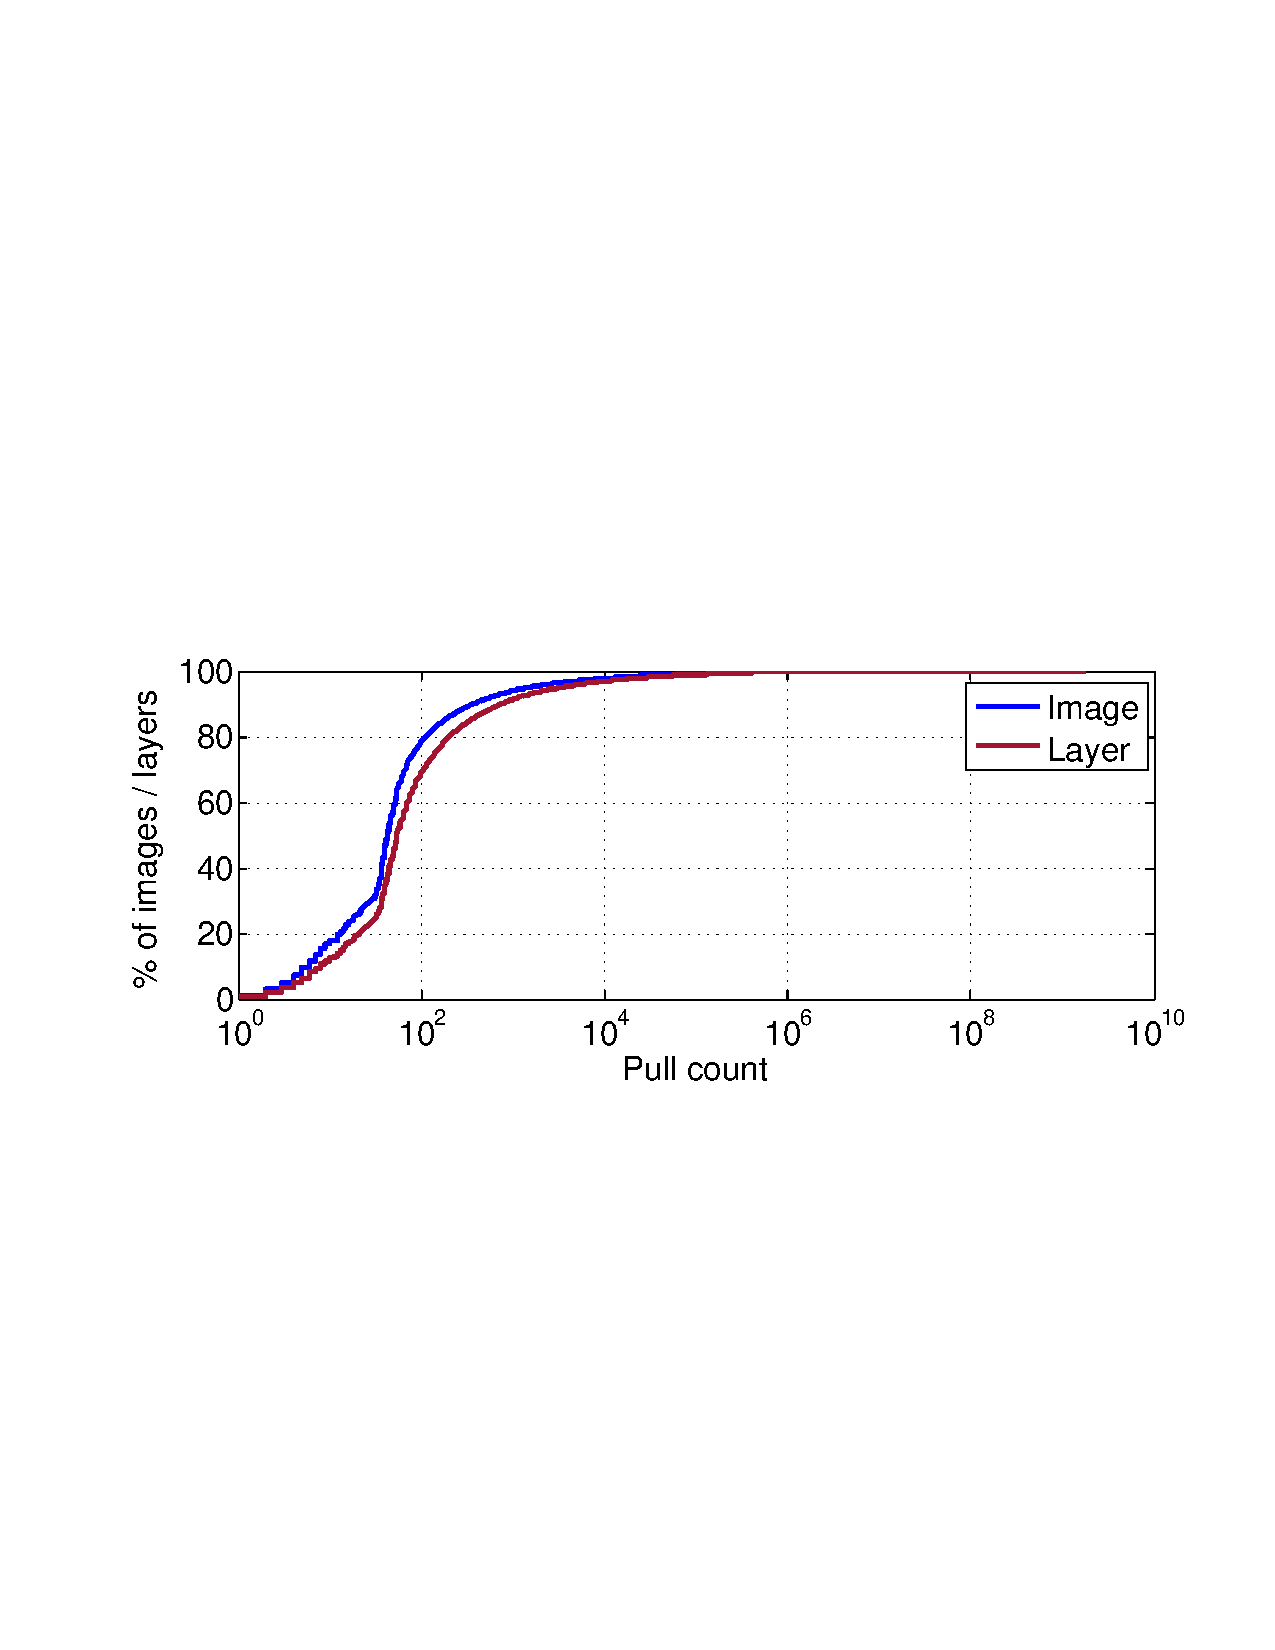
\includegraphics[width=0.4\textwidth]{graphs/pull-cnt.pdf}
	\caption{CDF of layer \& image pull count.
	}
	\label{fig:pull-cnt}
\end{figure}

\paragraph{Caching hot layers}

To further reduce overhead, we propose to cache the hot/recently requested layers as
gzip compressed tar files.
%
We observe that only a small proportion of images
and layers are frequently requested and majority of images and layers are
\textit{cold}.
%
Figure~\ref{fig:pull-cnt} shows the total
number of pulls from the time an image/layer has been stored in Docker Hub until
May 30, 2017.
%
We see that only 20\% and 10\% of images are pulled more than 100 and
360 times respectively.
%
Similarly, only 20\% and 10\% of layers are pulled
more than 217 and 660 times.
%
Note that we calculate the layer pull count shown in
Figure~\ref{fig:pull-cnt} by aggregating the pull count of
all images, which refer to this layer.
%
%Note that the image pull counts are crawled
%from Docker Hub website.
%
Actual layer pull counts should be less because pulling an image does not
necessarily pull all its containing layers if some layer have been previously
downloaded and are already available locally.
%

%
%\lrcomment{How does this compare to pulling without dedup? What's the overhead
%added?}


%
%\vcomment{What are the units for  $\sigma_{wl}$ and  $\sigma_{su}$?}
%
%\lrcomment{Do you mean it only runs through low workload periods? How are we
%predicting those or are we relying on some workload patterns? We should make
%that clear.}

%high while start file-level dedup \paragraph{\sysname\ model}
%Figure~\ref{fig:file-dedup-model} shows an example of \sysname\.
%
%\vcomment{An example?..}
%
%\lrcomment{This explanation should come before the caching and light workloads
%paragraphs.}
%

%\paragraph{Caching hot layers to improve performance}
%\label{subsec:\sysname\}
%
%\begin{figure}
%	\centering
%	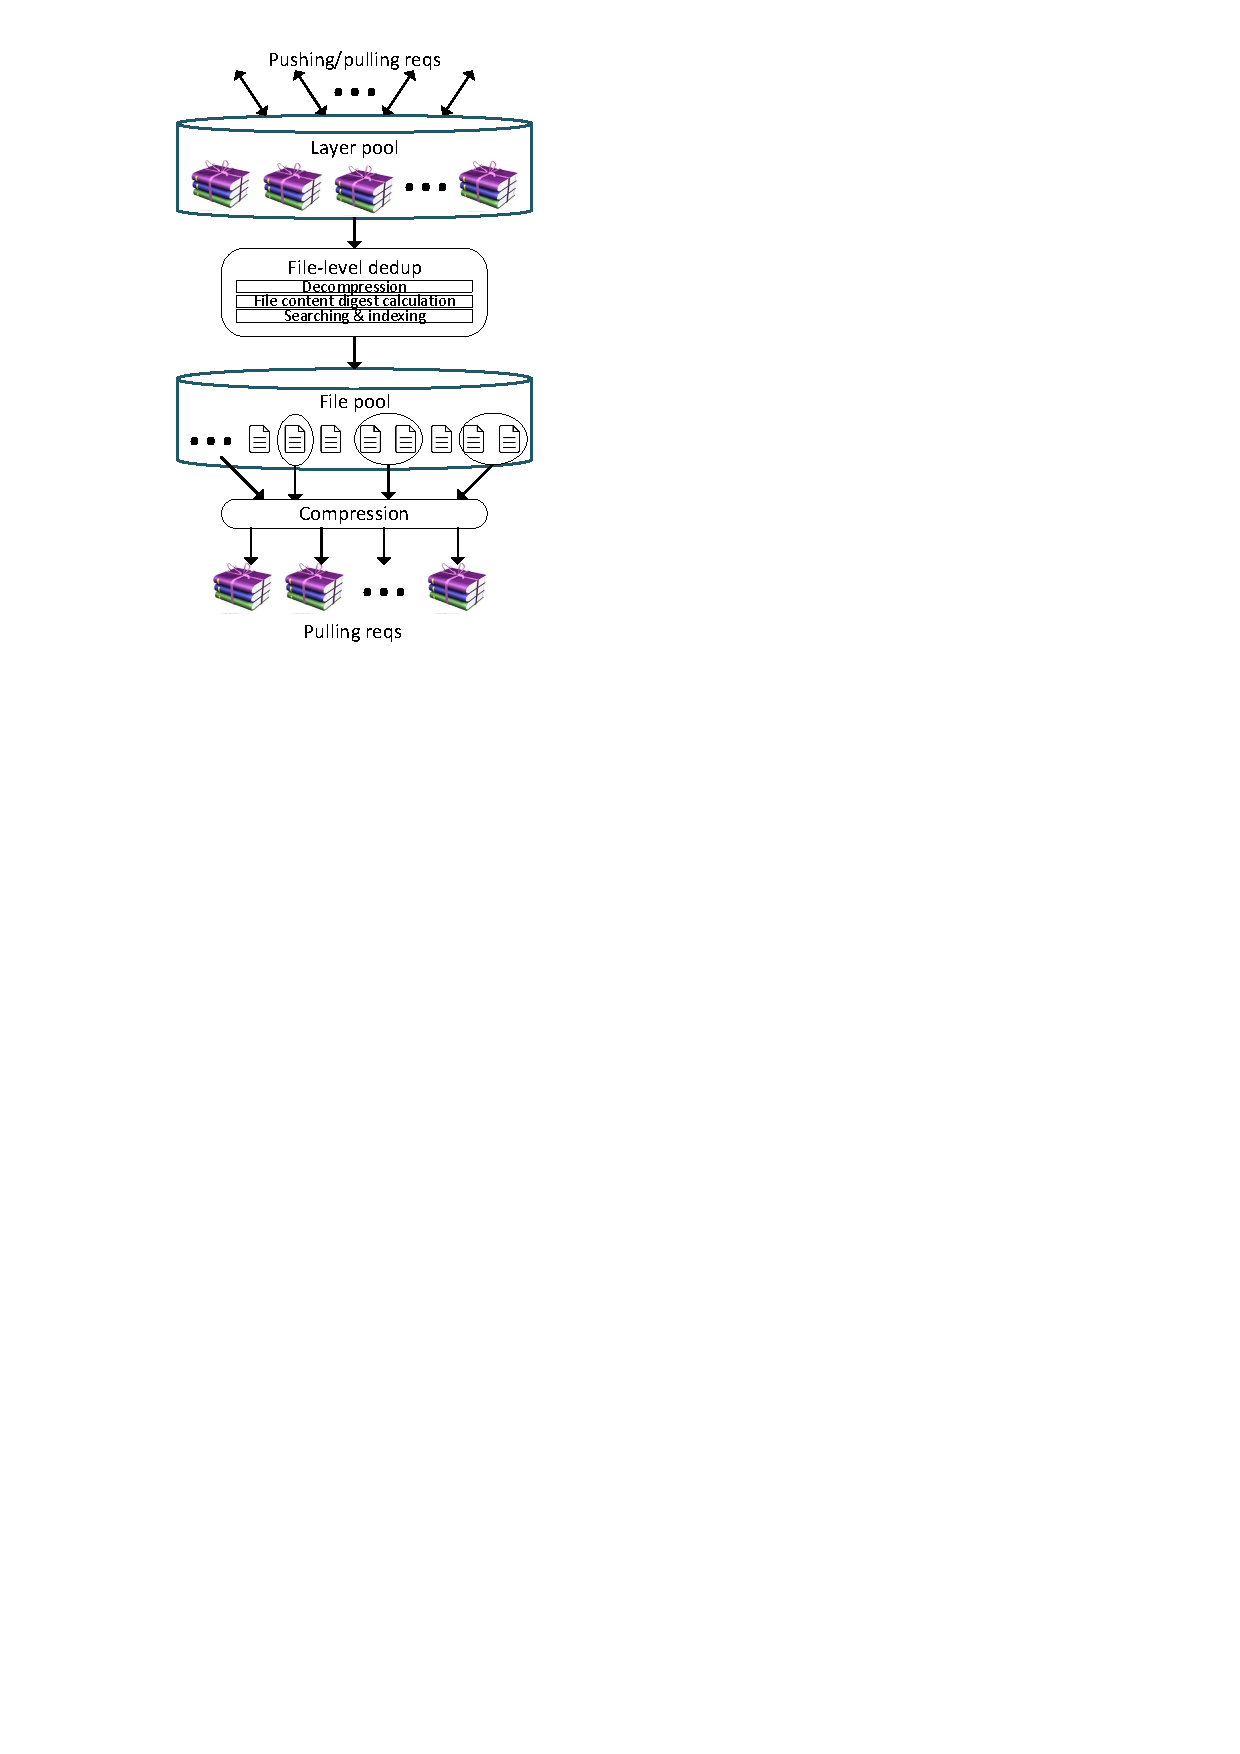
\includegraphics[width=0.3\textwidth]{graphs/graph_compression_layers.pdf}
%	\caption{File-level content addressable model.
%	\vcomment{1) Do not see ``cache'' word on the figure. 2) Font is too small in the middle section. 3) We need to describe how we depict layers vs. files. 4) There are pull requests both from the top and the bottom . I think we should just remove the part below the File pool.}
%	}
%	\label{fig:file-dedup-model}
%\end{figure}

%
%\vcomment{Who is ``it''?}\nancomment{addressed}
%
%
%\vcomment{Who are ``they''? Avoid using ``it'' and ``they''. Use actual nouns instead.}
%
 %a digest generated by a cryptographic hash function (such as ) 
%
%\vcomment{Let's use ``deduplication'' instead of ``dedup'' everywhere (because
%the letter one is informal)}

%\subsection{Trade-off discussion}

%

%\vcomment{I think there are two reasons for the cache 1) reduce push latency
%and 2) reduce pull latency. The text above talks only about reducing pull
%latencies.  We also need to talk about pushes.  Furthermore, the current
%discussion of pull counts does not really justify read (pull) cache.  For the
%read (pull) cache to be efficient there should be many pulls that access the
%same layers. E.g., that XXX\% of pulls go to the few YYY popular layers.
%Can we say that?}
%%
%\vcomment{somewhere we will need to talk about eviction policy, how to
%size the caching layer, and, finally, what happens if the cache is full.}
% 

%\subsection{Using RAM to load \&. process layers}
%
%To improve performance, we use RAM to temporarily store \textit{small} layers
%and directly process them in RAM.  Specially, we first load small layers in a
%RAM disk and perform decompression, unpacking, file content digest calculation
%in RAM, and remove them from RAM after completion.   According to our findings
%that majority (87.3\%) of layers that are less than 50M as shown in
%Figure~\ref{fig:image-layer-size}. So majority of layers can be stored and
%processed in RAM to speed up file-level dedup. 
%%layers that are less than 50M are stored and processed in RAM while the rest
%%layers are stored and processed in SSDs.
%%
%\lrcomment{This should still be part of 7.1 as it explains the strategy and not
%the prototype/simulations.}
%%
%\lrcomment{How are small layers defined? Where is the threshold?}
%
%majority (xxx) of layers'dedup times are less than xxx.
%during peak workload, which means that we start file-level dedup whenever it receives a layer. 
%To simulate the high intensive workload, we first sent a sequential of layer pushing requests to registry and stored, then we measure the file-level dedup  
%, archiving time, and compression time.
%Second, compare the latency for each operation, we see that xxxx
%\paragraph{Latency breakdown}
%We calculated the latency for each operation for all layers as shown as Table~\ref{tbl:latency_breakdown}.
%Figure~\ref{xxx} shows the compression time across 

%\begin{figure}[!t]
%	\centering
%	\subfigure[CDF of repositories by pull count]{\label{fig_pull_cnt_total}
%		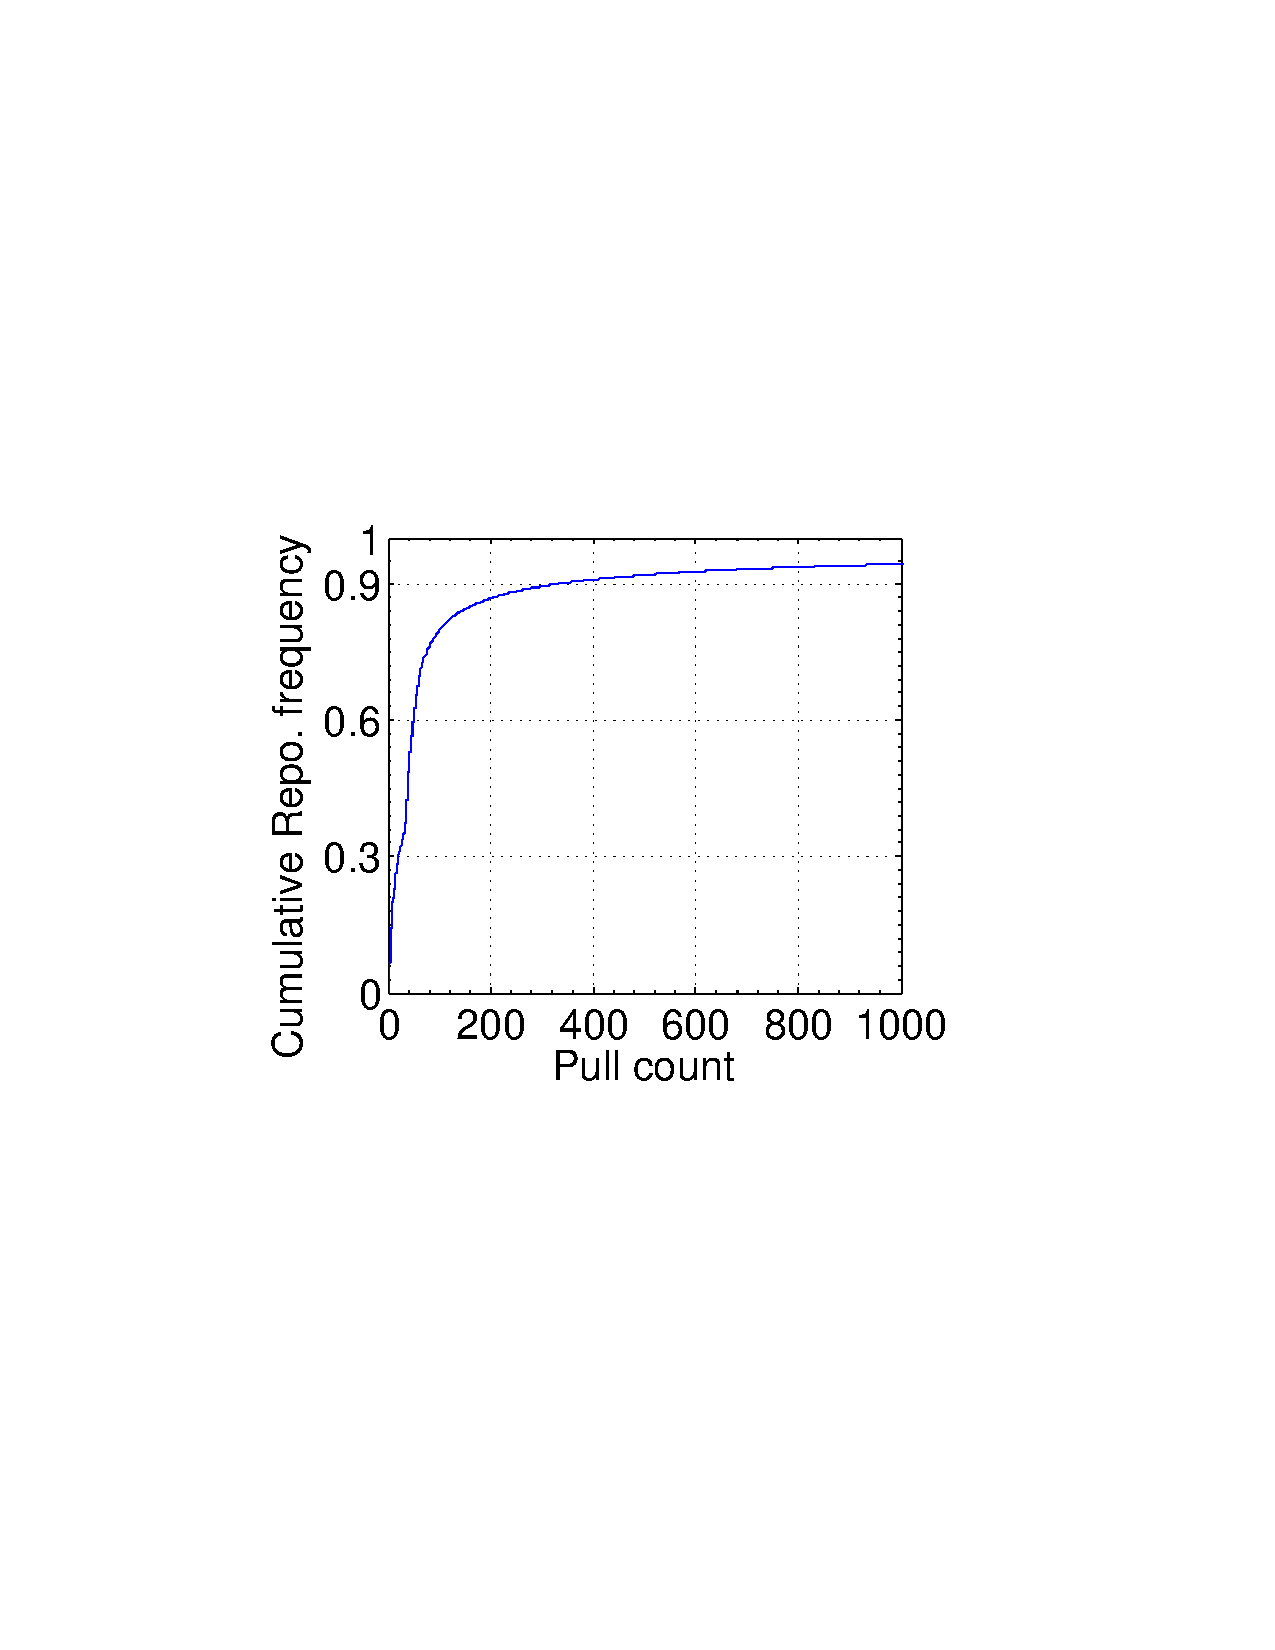
\includegraphics[width=0.23\textwidth]{graphs/pull_cnt.pdf}%
%	}
%	\subfigure[Histogram of repositories by pull count]{\label{fig_pull_cnt_count}
%		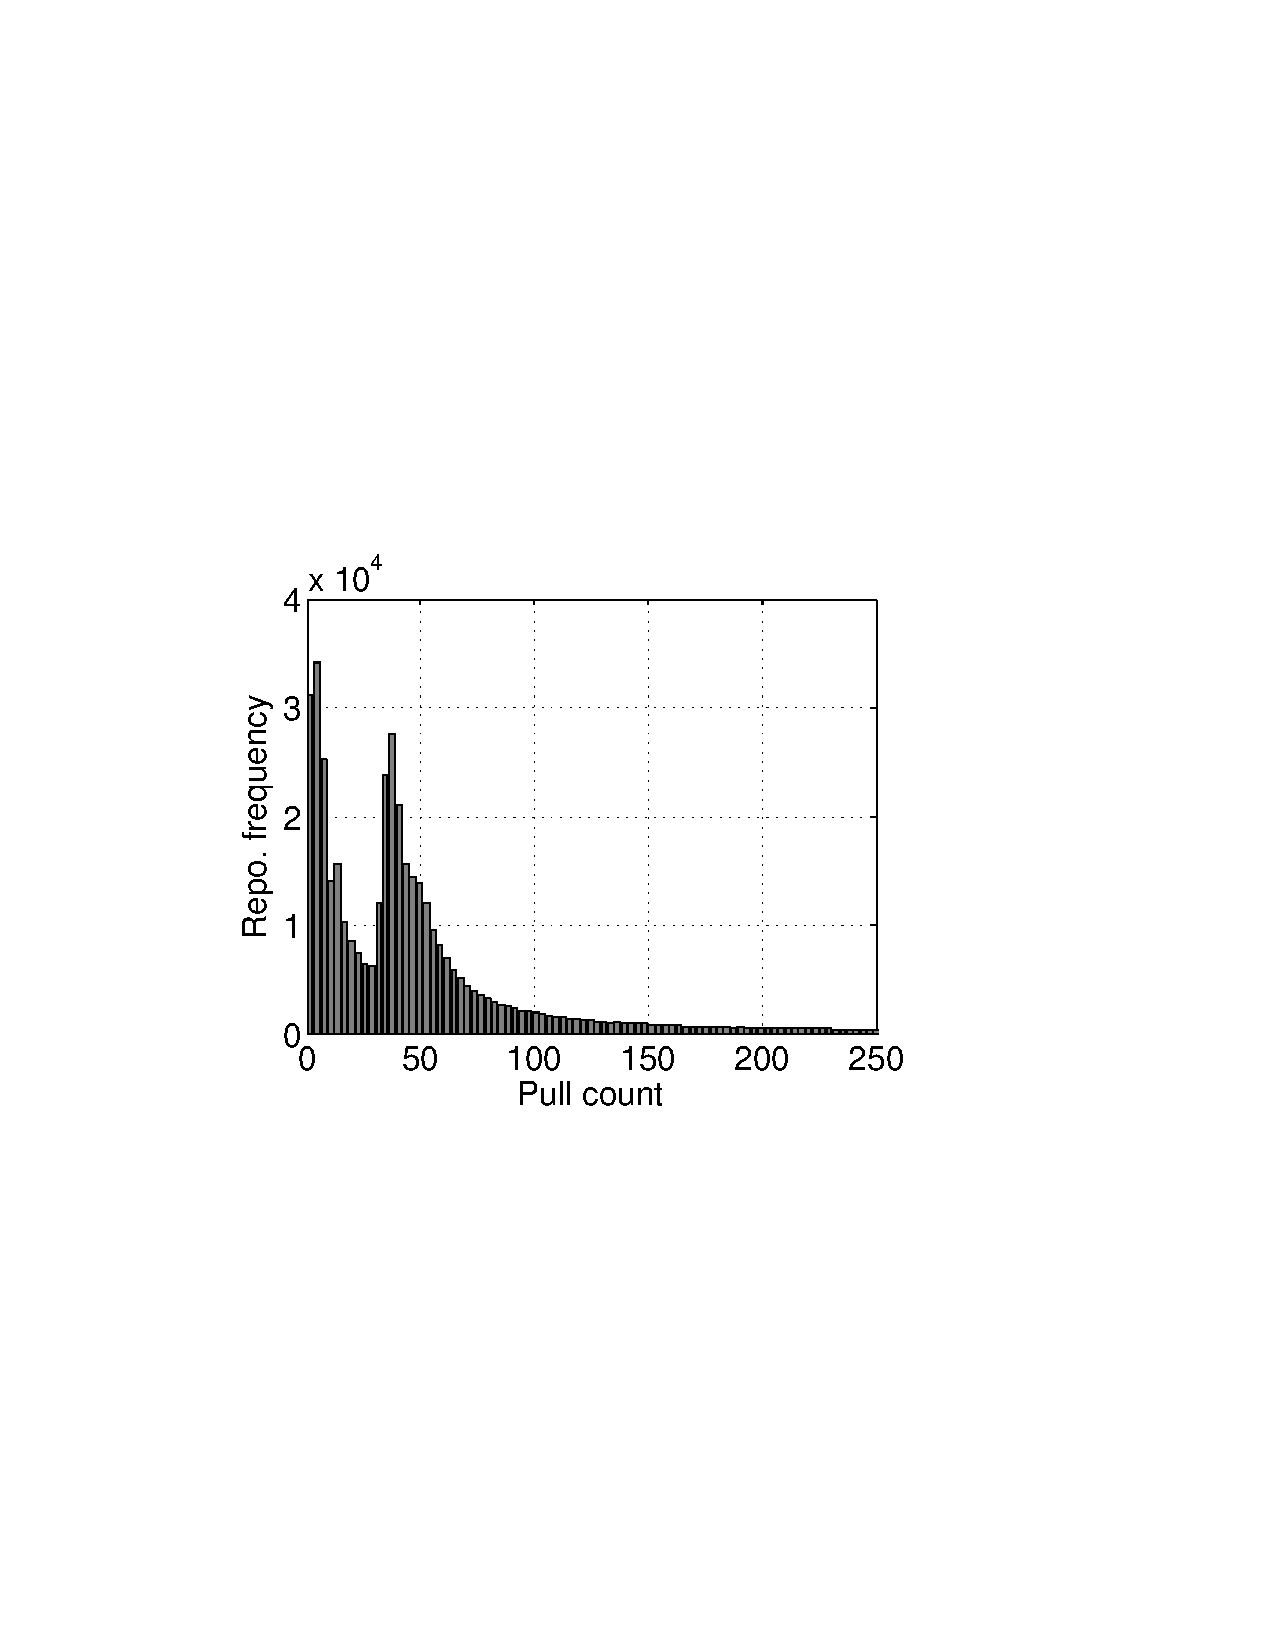
\includegraphics[width=0.22\textwidth]{graphs/count_pull_cnt.pdf}
%	}
%	\caption{Repository popularity distribution}
%	\label{fig-pop}
%\end{figure}

%=======================================
%|             OLD VERSION              |
%=======================================

%\paragraph{Latency distribution for each operation}
%\subsubsection{When to start file-level dedup?} 

%\paragraph{Latency distribution for each operation}

%\paragraph{Small compression ratio and small layer size}
%
%\begin{figure}[!t]
	\centering
	\subfigure[CDF of compression ratio]{\label{fig_cdf_compression_ratio}
		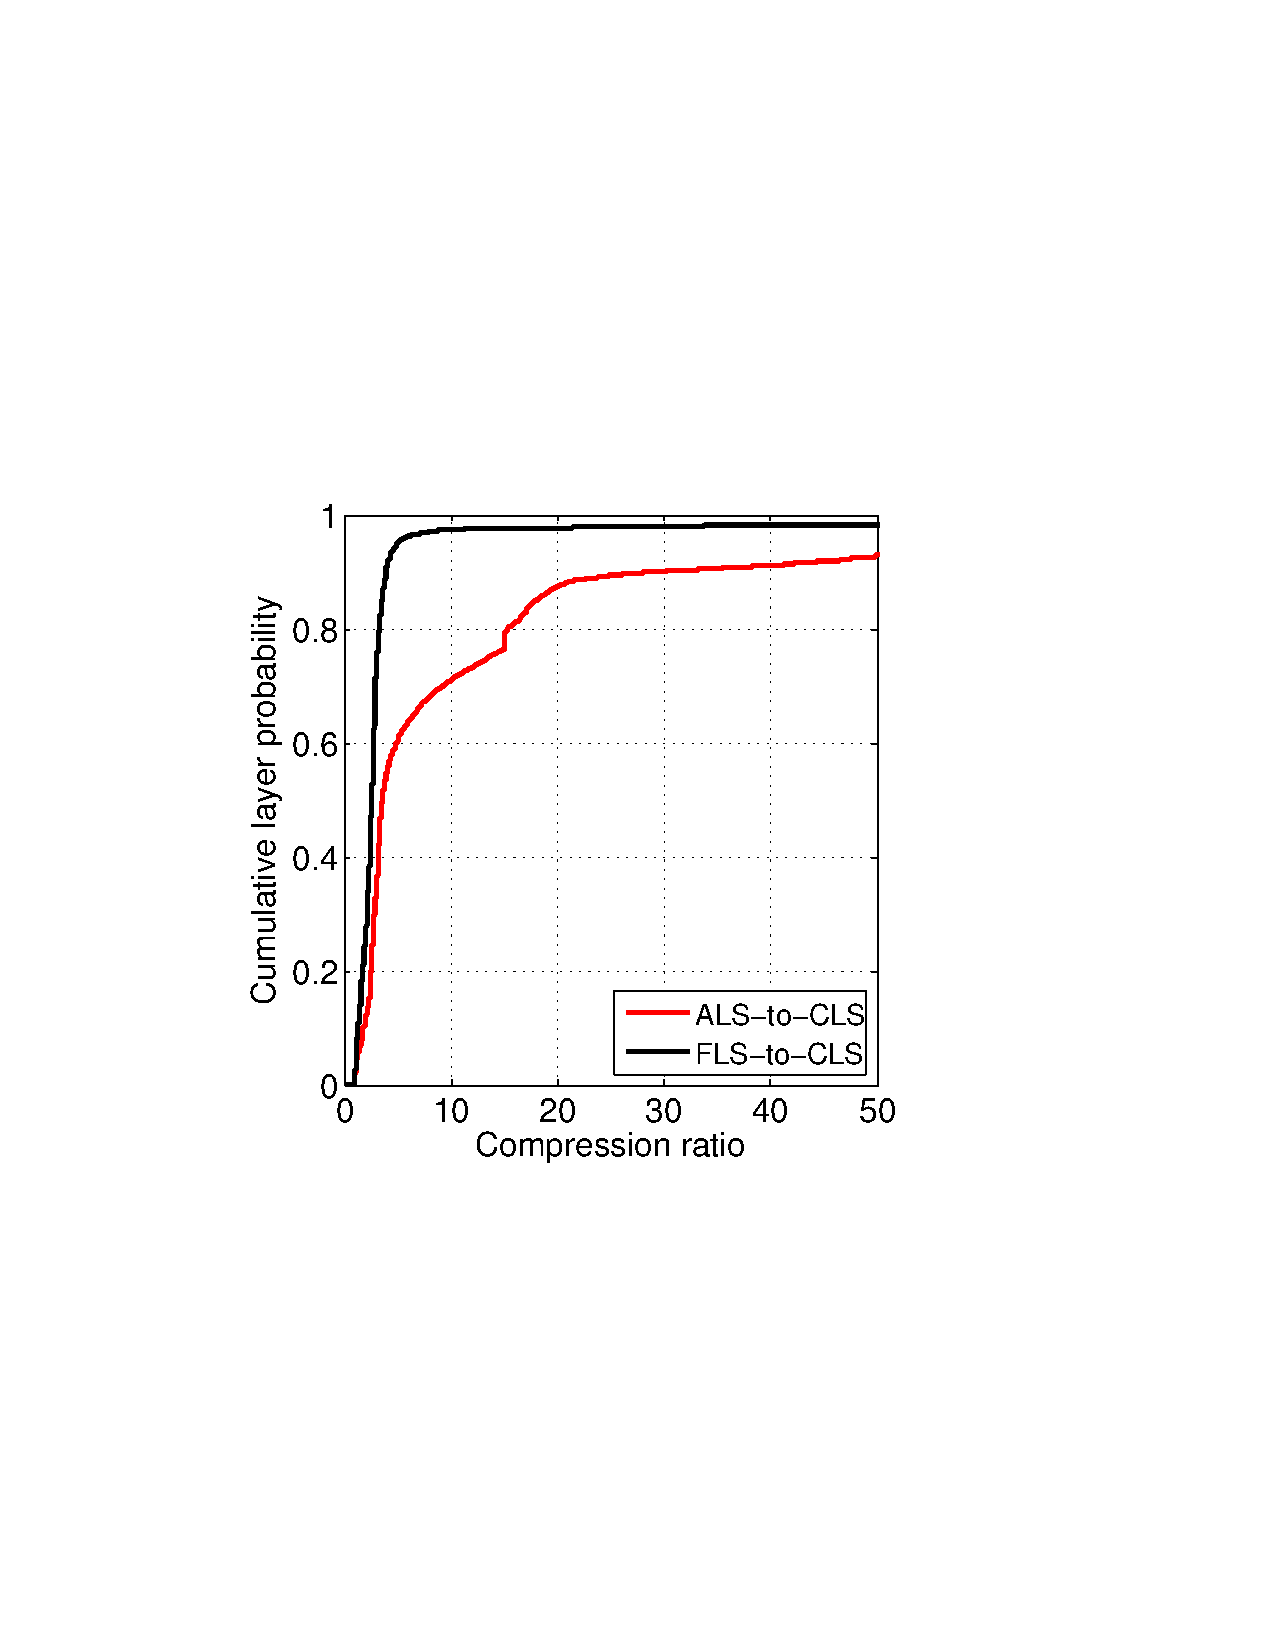
\includegraphics[width=0.23\textwidth]{graphs/cdf_compression_ratio.pdf}
	}
	\subfigure[Histogram of comp. ratios]{\label{fig_his_compression_ratio}
		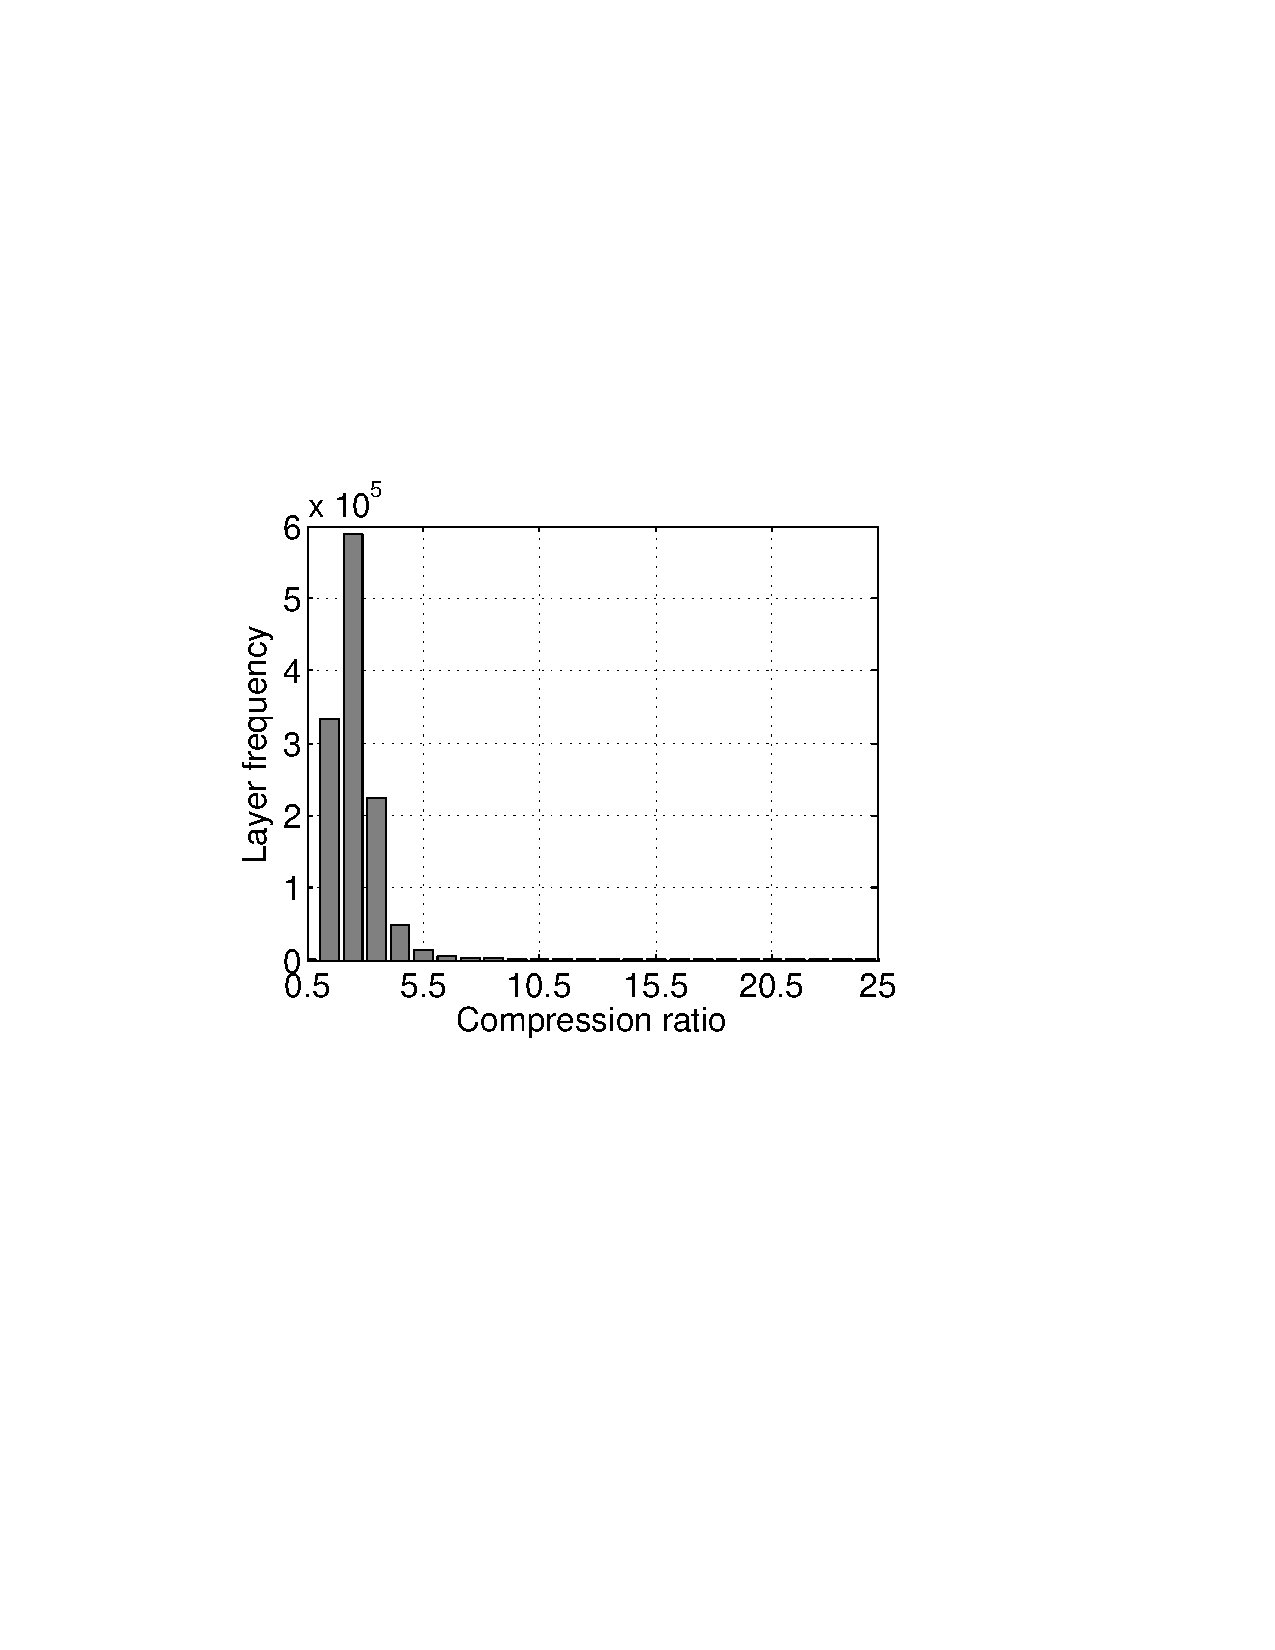
\includegraphics[width=0.223\textwidth]{graphs/his_compression_ratio.pdf}
	}
	\caption{Layer compression ratio distribution
	%\vcomment{Different colors are used in figure (a) and (b) FLS/CLS\nancomment{will address later}}
	}
	\label{fig-compression-ratio}
\end{figure}

%
%\begin{figure}[!t]
	\centering
	\subfigure[CDF of layer sizes]{\label{fig_layer_size_cdf}
		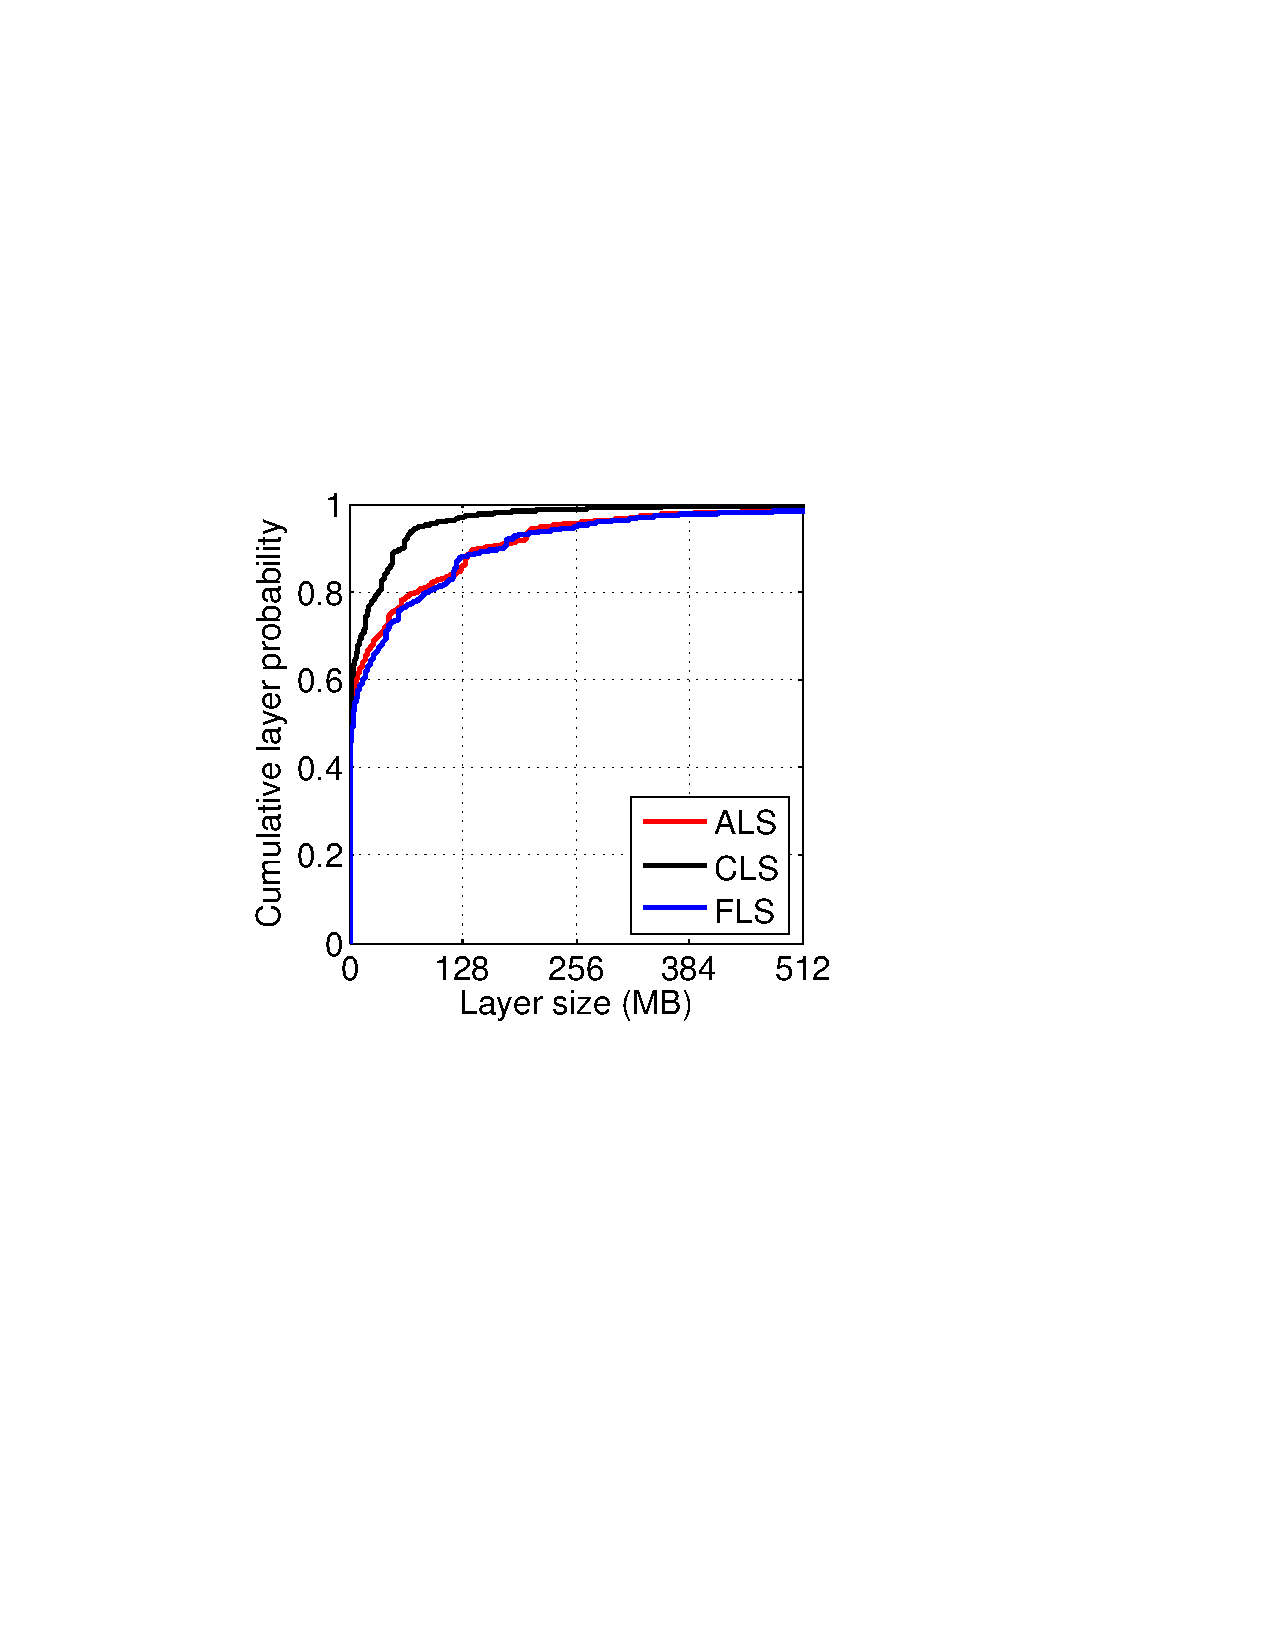
\includegraphics[width=0.234\textwidth]{graphs/layer_size_mb.pdf}
	}
	\subfigure[Histogram of layer sizes]{\label{fig_hist_layer_size}
		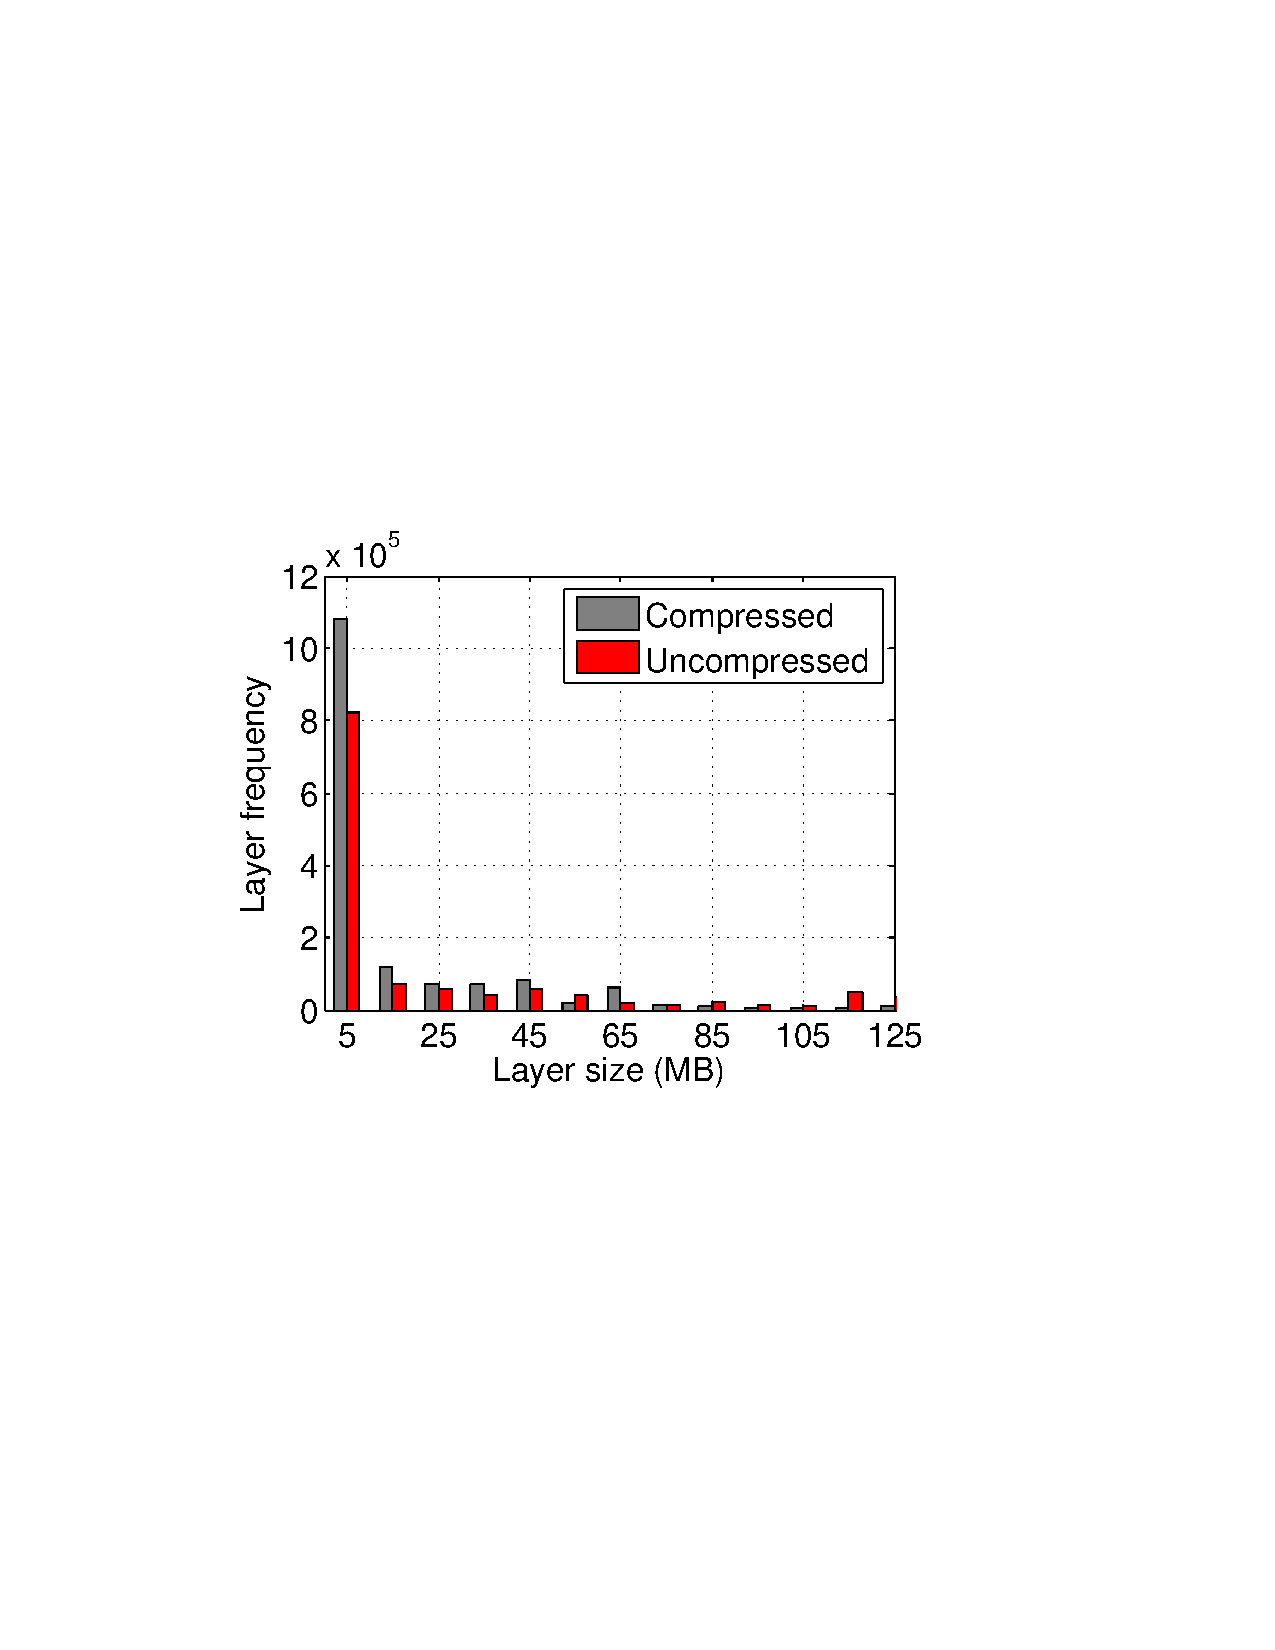
\includegraphics[width=0.213\textwidth]{graphs/hist_layer_size.pdf}
	}
	\caption{Layer size distribution
	\vcomment{Let's use CLS, ALS, and FLS abreviations\nancomment{addressed}}.
	\vcomment{CLS size should go first}.
	\vcomment{We need to use different types of lines (solid, dotted, etc.)
		or markers (round, triangular)}.
	\vcomment{In figure B it is not clear to which bar group corresponds
		  to which layer size. I suggest to try to rotate the graph
		  by 90 grads to fit all layer size labels.\nancomment{aligned label with bar}}
	}
	\label{fig-layer-size}
\end{figure}

%
%We found that most layers'compression ratio is really lower (?) while most of layers have a smaller size. 
%So how about we use archiving instead of compression if the network speed is higher (?GB/s)?

%\paragraph{Network transfer speed is high!}

%\subsubsection{File-level content addressable storage for cold layers}

%\begin{figure}
%	\centering
%	\includegraphics [width=0.45\textwidth]{plots/exp-total-stev-erase.eps}
%	\subfigure[]{\label{fig:per_layer_ratio_fcnt_cdf}
%		\includegraphics [width=0.23\textwidth]{graphs/}
%	}
%	\subfigure[Similar layer dedup]{\label{fig:per_layer_ratio_fcnt_pdf}
%		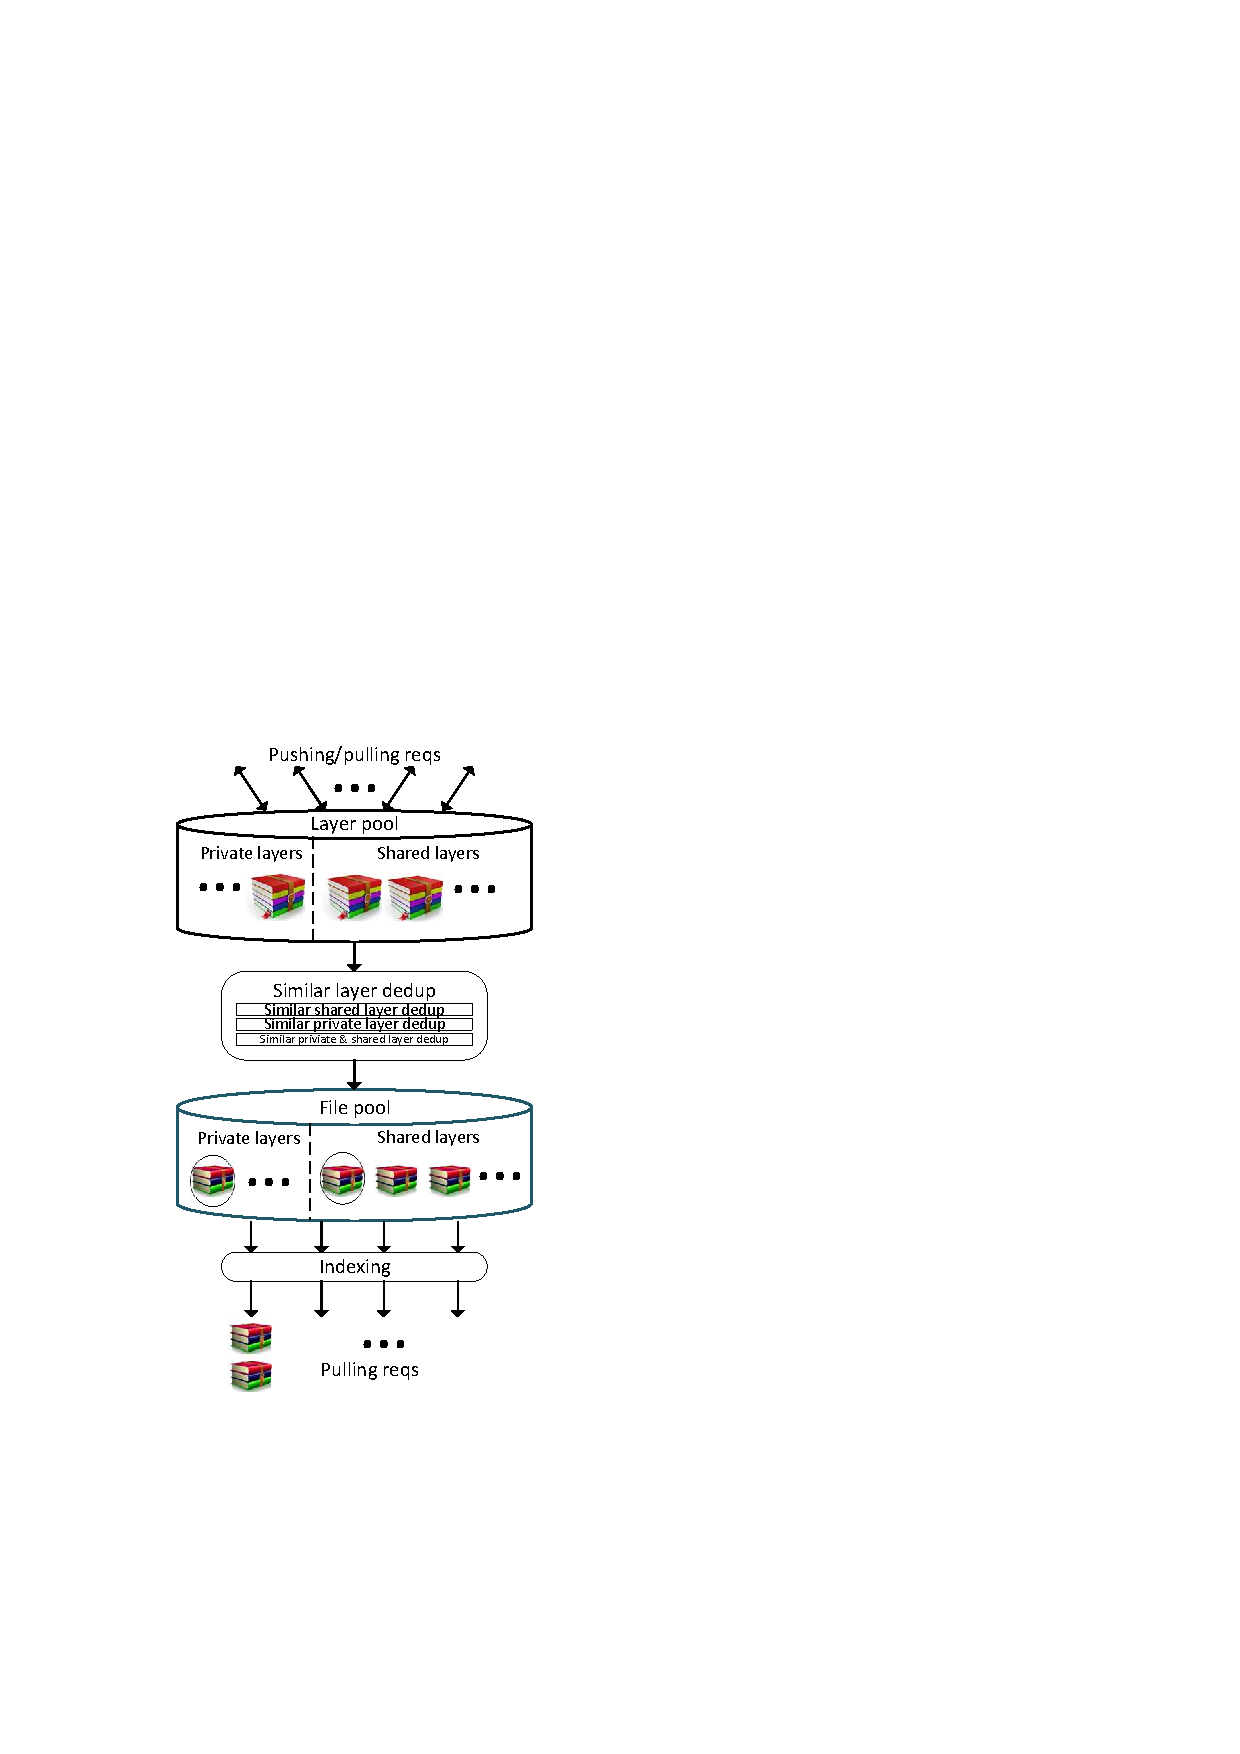
\includegraphics [width=0.22\textwidth]{graphs/graph_reconstruct_layers.pdf}
%	}
%	\caption{File-level content addressable storage model}
%	\label{fig:eval-stdev-erasure-cnt}
%\end{figure}

%\subsection{Hints for performance improvement and storage saving}

%\begin{table} 
%	\centering 
%	\scriptsize  
%	%\begin{minipage}{.5\linewidth}
%	\caption{Latency breakdown} \label{tbl:latency_breakdown} 
%	\begin{tabular}{|l|l|l|l|l|}%p{0.14\textwidth} 
%		\hline 
%		% after \\: \hline or \cline{col1-col2} \cline{col3-col4} ... 
%		% after \\: \hline or \cline{col1-col2} \cline{col3-col4} ... 
%		Operations/latency (S) & max & min & median & avg.\\
%		\hline
%		 gunzip decompression (RAM) & 257.16  & 0.04  & 0.15  & 0.39 \\
% 		\hline
% 		tar extraction (RAM) & 43.41  & 0.04  &  0.14  & 0.18 \\
%		\hline
%		Digest calculation (RAM) & 3455.01  & $<$0.00  & 0.05 & 10.65 \\
%		\hline
%		tar archiving (RAM)  & 53.44 & 0.04 & 0.14 & 0.19\\
%		\hline
%		gzip compression (RAM) & 496.04 & 0.04 & 0.15 & 2.10 \\
%%		\hline
%%		Total time (RAM) (with compression) & & & & \\
%%		\hline
%%		Total time (RAM) (without compression) & & & & \\
%		\hline
% 		\hline
% 		gunzip decompression (SSD) &   &   &    &  \\
% 		\hline
% 		tar extraction (SSD) &   &   &    &  \\
%		\hline
%		Digest calculation (SSD) &  &  & & \\
%		\hline
%		tar archiving (SSD) &  &  & & \\
%		\hline
%		gzip compression (SSD) & &  &  & \\
%%		\hline		 
%%		Total time (SSD) (with compression) & & & & \\
%%		\hline
%%		Total time (SSD) (without compression) & & & & \\
%		\hline
%		\hline
%		Network transfer & 20587.94 & $<$ 0.00 & $<$ 0.00 & 1.20 \\
%		\hline 	
%	\end{tabular} 
%\end{table}


%\begin{table} 
%	\centering 
%	\scriptsize  
%	%\begin{minipage}{.5\linewidth}
%	\caption{Summary of layer \& image characterization} \label{tbl:redundant_ratio} 
%	\begin{tabular}{|l|l|l|l|l|}%p{0.14\textwidth} 
%		\hline 
%		% after \\: \hline or \cline{col1-col2} \cline{col3-col4} ... 
%		% after \\: \hline or \cline{col1-col2} \cline{col3-col4} ... 
%		Metrics & max & min & median & avg.\\
%		\hline
%		Compressed layer size &   &   &   &  \\
%		\hline
%		Uncompressed layer size &   &   &    &  \\
%		\hline
%		Archival size &  &  & & \\
%		\hline
%		Compression ratio &   &   &    &  \\
%		\hline
%		Layer pull cnt. &  &  & & \\
%		\hline
%		File cnt. per layer &  &  & & \\
%		\hline
%		Dir. cnt. per layer &  &  & & \\
%		\hline
%		Layer depth &  &  & & \\
%		\hline
%		\hline
%		Compressed image size &  &  & & \\
%		\hline
%		Uncompressed image size & &  &  & \\
%		\hline
%		Archival image size & &  &  & \\
%		\hline
%		Compression ratio &   &   &    &  \\
%		\hline
%		Image pull cnt.  &  &  & & \\
%		\hline
%		Layer cnt. per image  &  &  & & \\
%		\hline
%		Shared layer cnt. per image  &  &  & & \\
%		\hline
%		File cnt. per layer &  &  & & \\
%		\hline
%		Dir. cnt. per layer &  &  & & \\
%		\hline	
%	\end{tabular} 
%\end{table} 

%\subsection{Constructing shared layers for redundant directories/files}
%
%\paragraph{Smaller number of layers are shared among different images}
%\begin{figure}[!t]
	\centering
	\subfigure[CDF of layer reference count]{\label{fig_repeate_layer}
		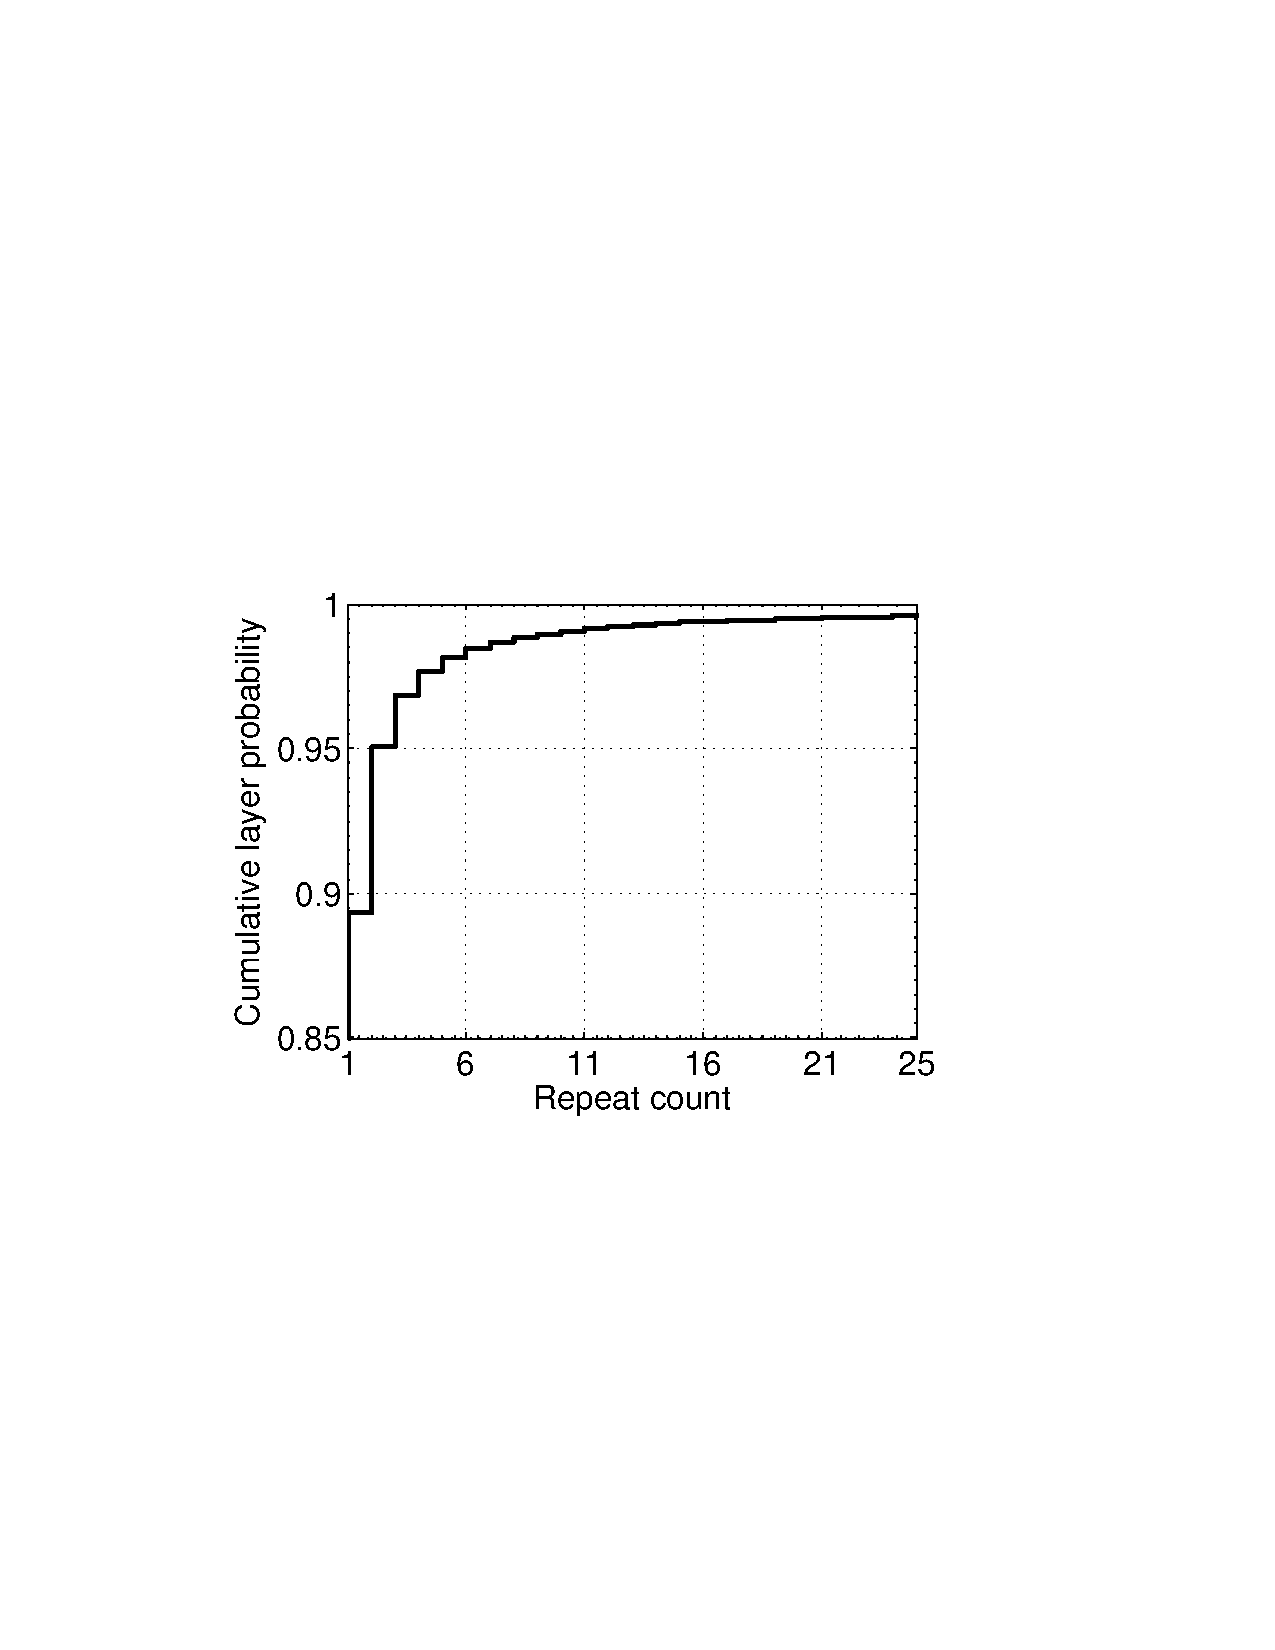
\includegraphics[width=0.23\textwidth]{graphs/repeate_layer.pdf}
	}
	\subfigure[Histogram of layer reference count]{\label{fig_hist_repeate_layer}
		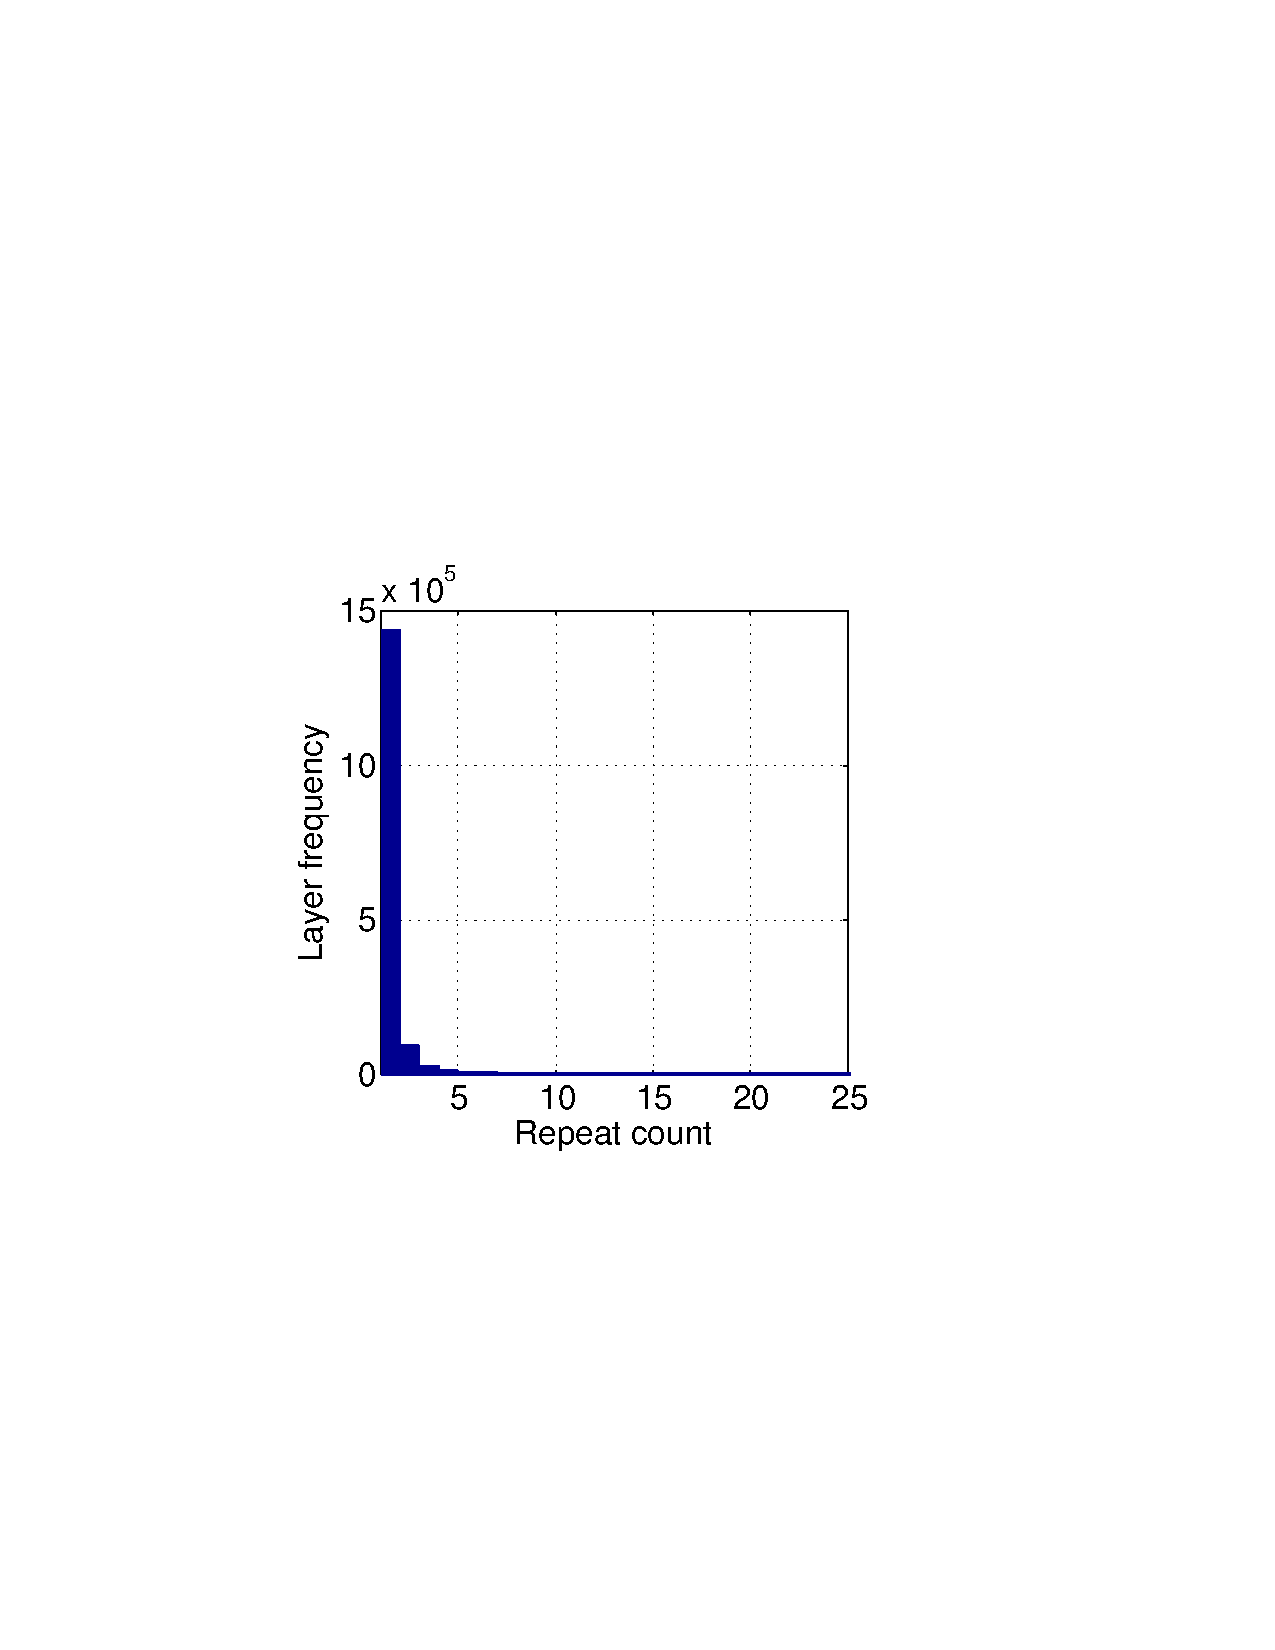
\includegraphics[width=0.223\textwidth]{graphs/hist_repeate_layer.pdf}
	}
	\caption{Layer reference counts across all images}
	\label{fig-repeat-layer-cnt}
\end{figure}
%
%\paragraph{Smaller pull latency than recompression model} the registry can prepare the reconstructed layers before users issue a pull request. But this model requires users to rebuild two layers.

%\subsubsection{Summary of Suggestions/trade-offs between dedup ratio and recompression overhead}
%
%\paragraph{1. using archiving instead of compression}
%\paragraph{2. using file-level dedup for cold images/layers}
%\paragraph{3. using file-level dedup economically}
%When to trigger file-level dedup?
%\paragraph{4. constructing shared layers for redundant dirs/files, for example,}
%%\subsection{Layer reconstruction model}
%%\subsubsection{Reconstruction overhead}
%%\subsubsection{Trade-offs between dedup ratio and reconstruction overhead}
%%\paragraph{Dedup ratio VS. Rebuild overhead}
%%\subsection{Evaluation results}
